\documentclass[11pt, a4paper]{article}
\usepackage{amsmath}
\usepackage[utf8]{inputenc}
\usepackage[brazilian]{babel}
\usepackage{graphicx}

\title{Dados sobre pessoas que viraram patos}
\author{João da Silva}

\begin{document}

  \maketitle

  \begin{tabular}{l c r}
    Ano & Número de pessoas que viraram patos & Pessoas felizes\\
    1990 & 101 & 550\\
    2000 & 557 & 2001\\
    2010 & 2734 & 17987\\
  \end{tabular}
  \\[1cm]
  \textbf{Obs:} o número de pessoas felizes é maior que o número de pessoas que se tornaram patos, pois os familiares das pessoas que se tornaram patos também ficaram felizes. Se tornar um pato é algo bom para toda a sociedade! (cf. também a Figura \ref{fig:graf_pato}).

  \begin{figure}[htb]
    \centering
    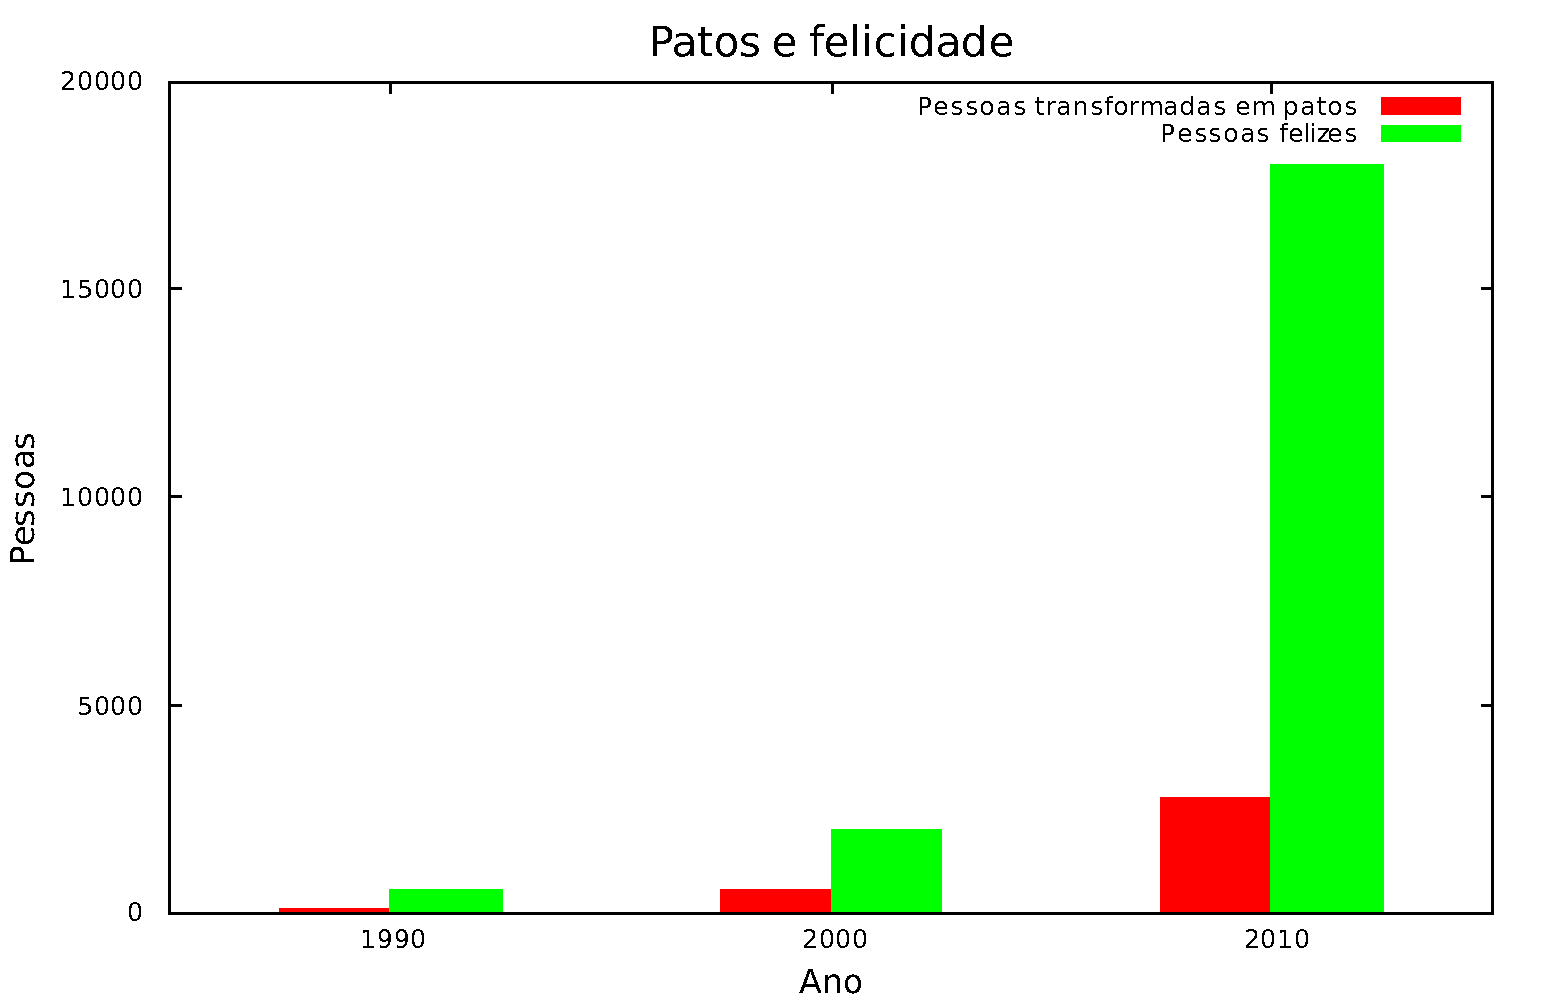
\includegraphics[width=\textwidth]{grafico_patos.pdf}
    \caption{Evolução recente do número de pessoas patonificadas e felicidade. Dados do último censo IBGE.}
    \label{fig:graf_pato}
  \end{figure}

\end{document}
